%!TEX TS-program = xelatex
\documentclass[12pt, a4paper, oneside]{article}

% Можно вставить разную преамбулу
% пакеты для математики
\usepackage{amsmath,amsfonts,amssymb,amsthm,mathtools}  
\mathtoolsset{showonlyrefs=true}  % Показывать номера только у тех формул, на которые есть \eqref{} в тексте.

\usepackage[british,russian]{babel} % выбор языка для документа
\usepackage[utf8]{inputenc}          % utf8 кодировка

% Основные шрифты 
\usepackage{fontspec}         
\setmainfont{Linux Libertine O}  % задаёт основной шрифт документа

% Математические шрифты 
\usepackage{unicode-math}     
\setmathfont[math-style=upright]{euler.otf} 

\setmathfont[range={\mathbb, \mathop, \heartsuit, \angle, \smile, \varheartsuit}]{Asana-Math.otf}

%%%%%%%%%% Работа с картинками и таблицами %%%%%%%%%%
\usepackage{graphicx} % Для вставки рисунков                
\usepackage{graphics}
\graphicspath{{images/}{pictures/}}   % папки с картинками

\usepackage[figurename=Картинка]{caption}

\usepackage{wrapfig}    % обтекание рисунков и таблиц текстом

\usepackage{booktabs}   % таблицы как в годных книгах
\usepackage{tabularx}   % новые типы колонок
\usepackage{tabulary}   % и ещё новые типы колонок
\usepackage{float}      % возможность позиционировать объекты в нужном месте
\renewcommand{\arraystretch}{1.2}  % больше расстояние между строками


%%%%%%%%%% Графики и рисование %%%%%%%%%%
\usepackage{tikz, pgfplots}  % языки для графики
%\pgfplotsset{compat=1.16}

\usepackage{todonotes} % для вставки в документ заметок о том, что осталось сделать
% \todo{Здесь надо коэффициенты исправить}
% \missingfigure{Здесь будет Последний день Помпеи}
% \listoftodos --- печатает все поставленные \todo'шки

\usepackage{multicol}

%%%%%%%%%% Внешний вид страницы %%%%%%%%%%

\usepackage[paper=a4paper, top=20mm, bottom=15mm,left=20mm,right=15mm]{geometry}
\usepackage{indentfirst}    % установка отступа в первом абзаце главы

\usepackage{setspace}
\setstretch{1.15}  % межстрочный интервал
\setlength{\parskip}{4mm}   % Расстояние между абзацами
% Разные длины в LaTeX: https://en.wikibooks.org/wiki/LaTeX/Lengths

% свешиваем пунктуацию
% теперь знаки пунктуации могут вылезать за правую границу текста, при этом текст выглядит ровнее
\usepackage{microtype}

% \flushbottom                            % Эта команда заставляет LaTeX чуть растягивать строки, чтобы получить идеально прямоугольную страницу
\righthyphenmin=2                       % Разрешение переноса двух и более символов
\widowpenalty=300                     % Небольшое наказание за вдовствующую строку (одна строка абзаца на этой странице, остальное --- на следующей)
\clubpenalty=3000                     % Приличное наказание за сиротствующую строку (омерзительно висящая одинокая строка в начале страницы)
\tolerance=10000     % Ещё какое-то наказание.

% мои цвета https://www.artlebedev.ru/colors/
\definecolor{titleblue}{rgb}{0.2,0.4,0.6} 
\definecolor{blue}{rgb}{0.2,0.4,0.6} 
%\definecolor{red}{rgb}{1,0,0.2} 
\definecolor{green}{rgb}{0, 0.6, 0}
\definecolor{purp}{rgb}{0.4,0,0.8} 

\definecolor{red}{RGB}{213,94,0}
\definecolor{yellow}{RGB}{240,228,66}


% цвета из geogebra 
\definecolor{litebrown}{rgb}{0.6,0.2,0}
\definecolor{darkbrown}{rgb}{0.75,0.75,0.75}

% Гиперссылки
\usepackage{xcolor}   % разные цвета

\usepackage{hyperref}
\hypersetup{
	unicode=true,           % позволяет использовать юникодные символы
	colorlinks=true,       	% true - цветные ссылки
	urlcolor=blue,          % цвет ссылки на url
	linkcolor=black,          % внутренние ссылки
	citecolor=green,        % на библиографию
	breaklinks              % если ссылка не умещается в одну строку, разбивать её на две части?
}

% меняю оформление секций 
\usepackage{titlesec}
\usepackage{sectsty}

% меняю цвет на синий
\sectionfont{\color{titleblue}}
\subsectionfont{\color{titleblue}}

% кружочки у цифр в секциях
\renewcommand{\thesection}{\arabic{section}}

% https://ru.overleaf.com/learn/latex/Sections_and_chapters

% выбрасываю нумерацию страниц и колонтитулы 
%\pagestyle{empty}

% синие круглые бульпоинты в списках itemize 
\usepackage{enumitem}

\definecolor{itemizeblue}{rgb}{0, 0.45, 0.70}

\newcommand*{\MyPoint}{\tikz \draw [baseline, fill=itemizeblue, draw=blue] circle (2.5pt);}
\renewcommand{\labelitemi}{\MyPoint}

\AddEnumerateCounter{\asbuk}{\@asbuk}{\cyrm}
\renewcommand{\theenumi}{\asbuk{enumi}}

% расстояние в списках
\setlist[itemize]{parsep=0.4em,itemsep=0em,topsep=0ex}
\setlist[enumerate]{parsep=0.4em,itemsep=0em,topsep=0ex}

% эпиграфы
\usepackage{epigraph}
\setlength\epigraphwidth{.6\textwidth}
\setlength\epigraphrule{0pt}

%%%%%%%%%% Свои команды %%%%%%%%%%

% Математические операторы первой необходимости:
\DeclareMathOperator{\sgn}{sign}
\DeclareMathOperator*{\argmin}{arg\,min}
\DeclareMathOperator*{\argmax}{arg\,max}
\DeclareMathOperator{\Cov}{Cov}
\DeclareMathOperator{\Var}{Var}
\DeclareMathOperator{\Corr}{Corr}

\DeclareMathOperator{\Pois}{Pois}
\DeclareMathOperator{\Geom}{Geom}
\DeclareMathOperator{\Exp}{Exp}

%\DeclareMathOperator{\E}{\mathbb{E}}
\DeclareMathOperator{\Med}{Med}
\DeclareMathOperator{\Mod}{Mod}
\DeclareMathOperator*{\plim}{plim}

% команды пореже
\newcommand{\const}{\mathrm{const}}  % const прямым начертанием
\newcommand{\iid}{\sim i\,i\,d\,\,}  % ну вы поняли...
\newcommand{\fr}[2]{\ensuremath{^{#1}/_{#2}}}   % особая дробь
\newcommand{\ind}[1]{\mathbbm{1}_{\{#1\}}} % Индикатор события
\newcommand{\dx}[1]{\,\mathrm{d}#1} % для интеграла: маленький отступ и прямая d

% одеваем шапки на частые штуки
\def \hb{\hat{\beta}}
\def \hs{\hat{s}}
\def \hy{\hat{y}}
\def \hY{\hat{Y}}
\def \he{\hat{\varepsilon}}
\def \hVar{\widehat{\Var}}
\def \hCorr{\widehat{\Corr}}
\def \hCov{\widehat{\Cov}}

% Греческие буквы
\def \a{\alpha}
\def \b{\beta}
\def \t{\tau}
\def \dt{\delta}
\def \e{\varepsilon}
\def \ga{\gamma}
\def \kp{\varkappa}
\def \la{\lambda}
\def \sg{\sigma}
\def \tt{\theta}
\def \Dt{\Delta}
\def \La{\Lambda}
\def \Sg{\Sigma}
\def \Tt{\Theta}
\def \Om{\Omega}
\def \om{\omega}

% Готика
\def \mA{\mathcal{A}}
\def \mB{\mathcal{B}}
\def \mC{\mathcal{C}}
\def \mE{\mathcal{E}}
\def \mF{\mathcal{F}}
\def \mH{\mathcal{H}}
\def \mL{\mathcal{L}}
\def \mN{\mathcal{N}}
\def \mU{\mathcal{U}}
\def \mV{\mathcal{V}}
\def \mW{\mathcal{W}}

% Жирные буквы
\def \mbb{\mathbb}
\def \RR{\mbb R}
\def \NN{\mbb N}
\def \ZZ{\mbb Z}
\def \PP{\mbb{P}}
\def \E{\mbb{E}}
\def \QQ{\mbb Q}

\def\F{\ensuremath{\mathcal{F}}} % аналогично!

%%%%%%%%%% Теоремы %%%%%%%%%%
\theoremstyle{plain} % Это стиль по умолчанию.  Есть другие стили.
\newtheorem{theorem}{Теорема}[section]
\newtheorem{proposition}{Утверждение}[section]
\newtheorem{result}{Следствие}[section]

% убирает курсив и что-то еще наверное делает ;)
\theoremstyle{definition}         
\newtheorem*{definition}{Определение}  % нумерация не идёт вообще


%%%%%%%%%% Задачки и решения %%%%%%%%%%
\usepackage{etoolbox}    % логические операторы для своих макросов
\usepackage{environ}
\newtoggle{lecture}

\newcounter{probNum}[section]  % счётчик для упражнений 
\NewEnviron{problem}[1]{%
    \refstepcounter{probNum}% увеличели номер на 1 
    {\noindent \textbf{\large \color{titleblue} Упражнение~\theprobNum~#1}  \\ \\ \BODY}
    {}%
  }

% Окружение, чтобы можно было убирать решения из pdf
\NewEnviron{sol}{%
  \iftoggle{lecture}
    {\noindent \textbf{\large Решение:} \\ \\ \BODY}
    {}%
  }
 
% выделение по тексту важных вещей
\newcommand{\indef}[1]{\textbf{ \color{green} #1}} 

% разные дополнения для картинок
\usetikzlibrary{arrows.meta}
\usepackage{varwidth}

\usepackage[normalem]{ulem}  % для зачекивания текста

% Если переключить в false, все solution исчезнут из pdf
\toggletrue{lecture}
%\togglefalse{lecture}



\title{
\begin{center} 
\includegraphics[width=0.99\textwidth]{logo.png}
\end{center}

Посиделка 2: как рождаются распределения}
\date{ } %\today}

% Если делаешь конспект, вписывай своё имя прямо сюда!
\author{Ульянкин Ппилиф}

\begin{document} % Конец преамбулы, начало файла

\maketitle

\epigraph{I am not in danger, Skyler. I am the danger! A guy opens his door and gets shot and you think that of me? No. I am the one who knocks!}{\textit{Walter White, Breaking Bad (2008-2013)}}


В этой лекции мы поговорим про ... 


\section{Варка распределений}

Давайте попробуем немного поработать с различными непрерывными распределениями. Пусть случайная величина $X$ имеет экспоненциальное распределение, $Exp(\alpha)$. То есть её функция распределения: 

$$
F_X(x) = \begin{cases} 1 - e^{-\alpha x}, &\text{ если } x \ge 0 \\ 0 &\text{ если } x < 0  \end{cases}
$$

А плотность:

$$
f_X(x) = \begin{cases} \alpha e^{- \alpha x}, &\text{ если } x \ge 0 \\ 0, &\text{ если } x < 0  \end{cases}
$$

Обычно с помощью такого распределения моделируют время между событиями. Например, время до следующего лайка под фотографией или время до прихода следующего человека в очередь. Почему именно с помощью него, мы узнаем чуть ниже. 

\textbf{Сейчас же давайте посмотрим на случайную величину $Y = \sqrt{X}$.} Нам нужно найти её плотность распределения. Разберёмся с областью определения новой случайной величины. Все значения $X$ лежат на полуинтервале $x \in [0; +\infty)$.  Получается, что для $Y$ будет выполнятся $y \in [\sqrt{0}; \sqrt{+\infty}) = [0; +\infty)$. 

Чтобы найти распределение $Y$ воспользуемся определением функции распределения: 

$$
F_Y(y) = \PP(Y \le y) = \PP(\sqrt{X} \le y) = \PP(X \le y^2) = F_X(y^2) = \begin{cases} 1 - e^{-\alpha y^2}, &\text{ если } y \ge 0 \\ 0, &\text{ если } y < 0  \end{cases}
$$

Вспоминаем, что $f_Y(y) = F'_Y(y)$ и добиваем задачу: 

$$
f_Y(y) = \begin{cases} 2 \cdot \alpha \cdot y \cdot e^{- y^2}, &\text{ если } x \ge 0 \\ 0, &\text{ если } x < 0  \end{cases}
$$

Ровно по такой же схеме можно пойти при работе с абсолютно любой функцией от случайной величины. 

\textbf{Посмотрим на ещё один пример $Y = 1 - e^{-\lambda X}$.} В качестве функции от $X$ мы берём её функцию распределения. Найдём область распределения новой случайной величины. Значения $X$ лежат на полуинтервале $x \in [0; +\infty)$. Найдём для нашей функции пределы при $x \to 0$ и $x \to +\infty$. Получим область определения для $Y$, $y \in [0; 1]$. 

Воспользуемся определением функции распределения

\begin{equation*}
F_Y(y) = \PP(Y \le y) = \PP(1 - e^{-X} \le y). 
\end{equation*}

Аккуратно раскроем неравенство под знаком вероятности

\begin{equation*}
    \begin{aligned}
        & 1 - y \le e^{-X} \\
        & \ln(1 - y) \le -X \\
        & X \le -\ln(1-y) \\
    \end{aligned}
\end{equation*}

Получим, что  

\begin{equation*}
\PP(1 - e^{-X} \le y) = \PP(X \le -\ln(1-y)) = F(-\ln(1-y)) = 1 - e^{\ln(1-y)} = 1 - 1 + y = y.
\end{equation*}

То есть

\begin{equation*}
F_Y(y) = \begin{cases} 1 \text{, если } y > 1 \\ y \text{, если } y \in [0; 1] \\ 0 \text{, если } y < 0.  \end{cases}
\end{equation*}

Взяв производную получим плотность распределения

\begin{equation*}
f_Y(y) = \begin{cases} 1 \text{, если } y \in [0;1]  \\ 0 \text{, если } x \notin [0;1].  \end{cases}
\end{equation*}

Эта плотность соответствует равномерному распределению на отрезке $[0;1]$. Выходит, что $Y = F_X(X) \sim U[0;1].$ Это неслучайный факт. Его обычно называют \indef{квантильным преобразованием}. Именно про него мы подробнее поговорим в следующем разделе. 

Здесь остаётся сказать, что приём, который мы использовали для получения новых распределений, довольно часто помогает получать распределения разных случайных величин. С его помощью можно получить распределение максимума и минимума из $n$ случайных величин. С помощью него можно вывести формулы для получения плотностей суммы, произведения и частного случайных величин. 

\section{Квантильное преобразование}

\begin{theorem} 
Пусть функция распределения $F_X(x)$ непрерывна. Тогда случайная величина $Y = F(X)$ имеет равномерное распределение на отрезке $[0; 1]$.
\end{theorem} 
\begin{proof} 
Чтобы доказать этот факт, просто-напросто воспроизведём логику из предыдущего раздела, но в более общем случае. Начнём с области определения $Y$. Это всегда отрезок $[0;1]$, так как именно на этом отрезке $F_X(x)$ принимает свои значения. 

Если функция распределения на всей своей области определения возрастает, значит она обратима, тогда: 

$$
F_Y(y) = \PP(F(X) < y) = \PP(X < F^{-1}(y)) = F(F^{-1}(y)) = y, \text{ если } x \in (0,1).
$$

При этом мы знаем, что функция распределения $F(y) = y$ соответствует равномерному на отрезке $[0;1]$ распределению. 

Если функция $F$ не является всюду возрастающей, то у неё есть участки постоянства. В этом случае просто обозначим через $F^{-1}(y)$ самую левую точку из замкнутого множества $\{t \mid F(t) = x\}$. При таком понимании обратной функции все равенства, перечисленные выше, остаются справедливы. 
\end{proof} 

\begin{result} 
Пусть $Y \sim U[0;1]$, а $F(x)$ произвольная функция распределения. Тогда случайная величина $X = F^{-1}(Y)$ будет иметь функцию распределения $F(x)$.
\end{result} 

Это следствие разрешает нам варить на компьютере любые случайные величины, для которых мы знаем $F_X(x)$. Нужно просто сгенерировать выборку из равномерного распределения, а затем применить к ней преобразование $F^{-1}(y)$. 

Например, если мы хотим получить выборку из экспоненциального распределения, $Exp(\alpha)$,  мы можем сделать это следующим образом: 

\begin{enumerate} 
\item Генерируем выборку $y_1, \ldots, y_n \sim \iid U[0;1]$
\item Находим выборку $x_1, \ldots, x_n$ по формуле: 

\[
x_i = F_X^{-1}(y_i) = -\frac{1}{\alpha} \ln(1-y_i).
\]
\end{enumerate} 

\begin{center} 
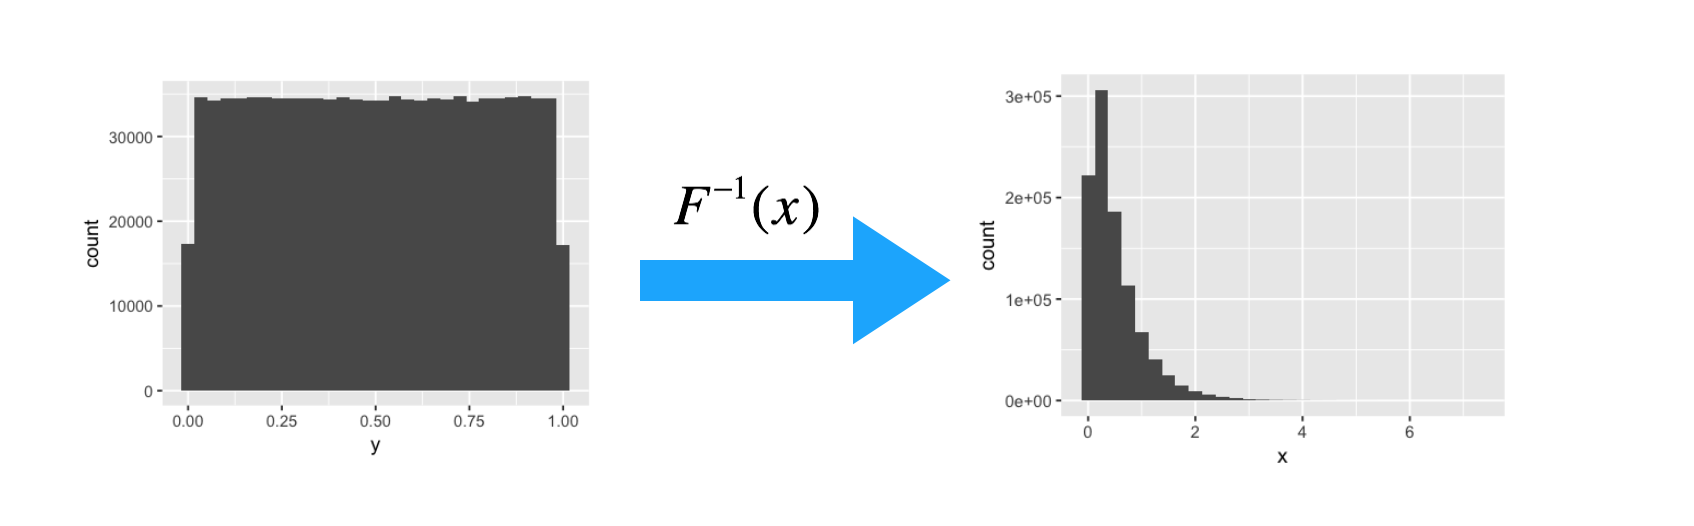
\includegraphics[width=0.98\linewidth]{pic_02_01.png}
\end{center} 

Для нормального распределения такой приём не сработает из-за того, что для него нет аналитической формулы для функции распределения из-за не берущегося интеграла. Для него приходится придумывать другие алгоритмы генерации. По аналогии для всех случайных величин, для которых функцию распределения нельзя записать в аналитическом виде, также придумывают свои методы генерации. На них мы посмотрим позже. 

\section{Большая сила о-малых}

Символом \indef{o-малое} обозначают любую бесконечно малую функцию $o(f(t))$ по сравнению с заданной функцией $f(t)$ при аргументе, стремящемся к некоторому конечному или бесконечному числу. 

Фраза <<функция $f(t)$ является o-малым от функции $g(t)$ в окрестности точки $t_0$>> означает, что с приближением $t$ к $t_0$ функция $f(t)$ уменьшается быстрее, чем $g(t)$. То есть отношение $\frac{g(t)}{f(t)}$ стремится к нулю. 

Математический анализ --- это тонкое искусство забивать. Обычно с помощью o-малых записывают то, на что можно забить. Например, пусть случайная величина $X$ имеет плотность распределения $f(t)$. Нам нужно примерно найти вероятность $\PP(X \in [t_0, t_0 + \Delta]).$

Предположим, что плотность выглядит как-то так: 

\begin{center} 
\begin{tikzpicture}
    \draw (-.2,4.8) node[left] {$f_X(t)$};
    \draw (6,-.5) node[below] {$t$};
    \draw[->] (0,0) -- (6.2,0) node[right] {};
    \draw[->] (0,0) -- (0,5) node[above] {};

    \def\gauss{\x,{4*1/exp(((\x-3)^2)/2)}}
    \draw[color=blue,domain=0:6] plot (\gauss) node[right] {};
 
    \def\y{2.7}
    \def\x{1.4}
    \def\fy{4*1/exp(((\y-3)^2)/2)}
    \def\fx{4*1/exp(((\x-3)^2)/2)}
 
    \fill [fill=orange!60] ({\x},0) -- plot[domain={\x}:{\y}] (\gauss) -- ({\y},0) -- cycle;
 
    \draw[dashed] ({\y},{\fy}) -- ({\y},0) node[below right] {$t_0 + \Delta$};
    \draw[dashed] ({\x},{\fx}) -- ({\x},0) node[below] {$t_0$};
    \draw[dashed] ({\x},{\fx}) -- ({\y},{\fx}) node[above left] {$o(\Delta)$};
    % \draw[dashed] ({\x},{\fx}) -- ({\y},{\fx}) node[below] {$S$};
\end{tikzpicture}
\end{center} 

Вероятность попасть в отрезок --- это площадь под плотностью. Величина $\Delta \cdot f(t_0)$ --- часть этой площади. Понятное дело, что это не вся площадь. Есть кусочек, который мы не учли. При маленьком $\Delta$ неучтённый кусочек будет очень маленьким и мы можем мм пренебречь. Обычно этот факт записывают с помощью о-малой

\[
\PP(X \in [t_0, t_0 + \Delta] = \Delta \cdot f(t_0) + o(\Delta).
\]

Если мы откинем её, точность немного пострадает. Обращаю ещё раз ваше внимание на то, что так можно делать только при очень маленьких $\Delta$. 

Несколько важных свойств: 

\begin{itemize} 
    \item Сколько о-малые не складывай, всё-равно получишь о-малую 
    
    \[o(\Delta) + o(\Delta) = o(\Delta).\]
    
    \item Сколько не умножай о-малую на число, больше она не станет
    
    \[o(5\Delta) = o(\Delta), \quad -o(\Delta) = o(\Delta). \]

\end{itemize} 

Дальше большая сила о-малых поможет нам аккуратно построить пуассоновский поток. 

\section{Пуассоновский поток из воздуха}

Поговорим про \indef{распределение Пуассона.} Обычно с помощью него моделируют простейший поток событий. Правда не очень понятно почему. Давайте по аналогии с нормальным распределением, выпишем несколько аксиом и затем попробуем получить из них распределение Пуассона. 

Даша выложила свою фотку и ждёт лайков. Лайки прилетают. Пусть $X_t$ --- число лайков, которое она получила за время $[0; t]$. Это дискретная случайная величина. В свою очередь, $Y_n$ --- время, которое прошло между $n-1$ и $n$ лайками. 

\begin{center} 
\begin{tikzpicture}[scale=2]
    \draw[->, very thick] (0,0) -- (6.2,0) node[right] {};
    \draw (6,-.1) node[below] {$t$};
    \draw (0,-.1) node[below] {$0$};
    
    \foreach \Point in {(0.5,0.1), (1,0.1), (2,0.1), (4,0.1), (4.5,0.1)}{
        \node at \Point {\color{red} \Large $\varheartsuit$};
    }
\end{tikzpicture} 
\end{center} 

Чтобы понять как именно распределены $X_t$ и $Y_n$ введём несколько аксиом о том, как ведёт себя поток лайков. 

\begin{enumerate} 
\item[\boxed{$PA-0$}] За нулевой промежуток времени мы всегда получаем ноль лайков, то есть $\PP(X_0 = 0) = 1$.

\item[\boxed{$PA-1$}] \indef{Отсутствия после действия:} вероятность появления $k$ событий на любом промежутке времени не зависит от того, сколько событий произошло до этого. 

То есть, если у нас есть промежутки $\Delta t$ и $\Delta s$, то $X_{\Delta t}$ и  $X_{\Delta s}$ не зависят друг от друга. Случайная величина $X_{\Delta t}$ описывает сколько лайков мы получили за промежуток времени $\Delta t$. 

\begin{center} 
\begin{tikzpicture}[scale=2]
    \draw[->, very thick] (0,0) -- (6.2,0) node[right] {};
    \draw (6,-.1) node[below] {$t$};
    \draw (0,-.1) node[below] {$0$};
    
    \draw[<->] (0.5,0.5) -- (2.5,0.5) node[right] {};
    \draw[<->] (3.5,0.5) -- (5.5,0.5) node[right] {};
    \draw (0.5,0.6) node[above] {$s_1$};
    \draw (2.5,0.6) node[above] {$s_2$};
    \draw (1.5,0.6) node[above] {$X_{\Delta s}$};
    \draw (3.5,0.6) node[above] {$t_1$};
    \draw (5.5,0.6) node[above] {$t_2$};
    \draw (4.5,0.6) node[above] {$X_{\Delta t}$};
    
    \foreach \Point in {(0.5,0.1), (1,0.1), (2,0.1), (4,0.1), (4.5,0.1)}{
        \node at \Point {\color{red} \Large $\varheartsuit$};
    }
\end{tikzpicture} 
\end{center} 

\item[\boxed{$PA-2$}] \indef{Стационарность:} появление $k$ событий на каком-то промежутке зависит только от числа $k$ и от длины этого промежутка. Точка начального отсчёта не имеет значения. 

То есть, интенсивность лайков постоянна во времени. Если у нас было два промежутка длиной в час, в разное время суток, то на этих двух промежутках появление $k$ лайков равновероятно. 

\item[\boxed{$PA-3$}] \indef{Ординарность:} наступление более одного события этого потока за бесконечно малый промежуток времени является практически невозможным.

Если $\Delta t$ очень маленькое, в течение него вероятность получить $1$ лайк пропорциональна $\Delta t$

$$
\PP(X_{\Delta t} = 1) = \lambda \cdot \Delta t + o(\Delta t).
$$

Вероятность получить один лайк линейно зависит от промежутка времени.Она существенно выше вероятности получить $2$ лайка и более

$$
\PP(X_{\Delta t} \ge 2) = o(\Delta t).
$$

Под $o(\Delta t)$ в лучших традициях матана подразумевается что-то очень маленькое. То, на что можно легко забить.  Величину $\lambda$ обычно называют \indef{интенсивностью потока событий.} Вероятность получить лайки определяется ей и промежутком времени. Поток событий, который подчиняется перечисленным аксиомам, называют \indef{простейшим потоком событий.}
\end{enumerate}

\textbf{Давайте найдём отталкиваясь от этих аксиом $\PP(X_t = k).$}  Для начала выпишем вероятность того, что за очень маленький промежуток времени мы не получим ни одного лайка. В этом нам поможет аксиома \boxed{$PA-3$}

\begin{multline*}
\PP(X_{\Delta t} = 0) = 1 - \PP(X_{\Delta t} = 1) - \PP(X_{\Delta t} = 2) - \PP(X_{\Delta t} = 3) - \ldots = \\ = 1 - (\lambda \cdot \Delta t + o(\Delta t)) - o(\Delta t) - o(\Delta t) - o(\Delta t) - \ldots = 1 - \lambda \cdot \Delta t + o(\Delta t).
\end{multline*}

Давайте попробуем рассмотреть число событий, которое произошло за промежуток времени $[0;t]$ и число событий, которое произошло за промежуток времени $\Delta t$.  \textbf{Обозначим вероятность того, что за промежуток $[0;t]$ не произойдёт ни одного лайка как $h_0(t) = \PP(X_t = 0)$.} Нам хочется понять как связаны между собой $h_0(t), h_0(\Delta t)$ и $h_0(t + \Delta t)$. 


\begin{center} 
\begin{tikzpicture}[scale=2]
    \draw[->, very thick] (0,0) -- (5,0) node[right] {};
    \draw (5,-.1) node[below] {$t + \Delta t$};
    \draw (4,-.1) node[below] {$t$};
    \draw (0,-.1) node[below] {$0$};
    
    \draw[<->, thick] (0,0.3) -- (3.9,0.3) node[right] {};
    \draw[<->, thick] (4.1,0.3) -- (5,0.3) node[right] {};
    \draw (2, 0.4) node[above] {$t$};
    \draw (4.5, 0.4) node[above] {$\Delta t$};
\end{tikzpicture} 
\end{center} 

По аксиоме \boxed{$PA-1$} число событий, произошедшее за промежутки $t$ и $\Delta t$ не зависят, так как промежутки не пересекаются.

\begin{itemize} 
\item  $h_0(t) = \PP(X_t = 0)$ --- вероятность того, что за время $t$ мы не получили ни одного лайка. 

\item $h_0(\Delta t) = \PP(X_{\Delta t} = 0)$ --- вероятность того, что за время $\Delta t$ мы не получили ни одного лайка. 

\item $h_0(t + \Delta t) = \PP(X_{t + \Delta t} = 0)$ --- вероятность того, что мы не за один из двух промежутков не получим лайк. 
\end{itemize} 

Получается, что в силу независимости событий, вероятность их произведения равно произведению их вероятностей: 

\[
h_0(t + \Delta t) = h_0(t) \cdot h_0(\Delta t).
\]

Мы хотим понять как выглядит функция $h_0(t).$ У нас есть значение функции в точке $t$, а ещё есть приращение $\Delta t$. Это всё жутко напоминает производную. Давайте попробуем свести получившееся уравнение к дифуру. 

Вычтем из обоих частей $h_0(t)$ и поделим их на $\Delta t$. Потом можно будет устремить $\Delta t$ к нулю и получить дифур

\begin{equation*}
\begin{aligned} 
    & \frac{ h_0(t + \Delta t) - h_0(t)}{\Delta t} = \frac{h_0(t) \cdot h_0(\Delta t) - h_0(t)}{\Delta t} \\
    & \frac{ h_0(t + \Delta t) - h_0(t)}{\Delta t} = \frac{h_0(t) \cdot( h_0(\Delta t) - 1)}{\Delta t}. \\
\end{aligned}
\end{equation*}

В правой части $h_0(t)$ никак не зависит от $\Delta t$. Если мы устремим $\Delta t \to 0,$ её можно вынести за знак предела. Для того, чтобы понять что происходит с оставшейся дробью, воспользуемся аксиомой  \boxed{$PA-3$} и распишем вероятность $h_0(\Delta t)$

\[
\frac{ h_0(\Delta t) - 1}{\Delta t} = \frac{ 1 - \lambda \Delta t + o(\Delta t) - 1}{\Delta t} = - \lambda  + \frac{o(\Delta t)}{\Delta t} \to -\lambda.
\]

Получаем уравнение 

\[
h_0'(t) = -\lambda \cdot h_0(t).
\]

Хм... Производная функции с точностью до константы равна самой функции... Попахивает экспонентой. Решим дифур: 

\begin{equation*}
\begin{aligned} 
    & \frac{\dx{h_0}}{\dx{t}} = -\lambda \cdot h_0 \\
    & \frac{\dx{h_0}}{h_0} = -\lambda \cdot \dx{t} \\
    & \ln h_0 = -\lambda t + \ln \const \\
    & h_0(t) = \const \cdot e^{-\lambda \cdot t}. \\
\end{aligned}
\end{equation*}

Найти константу можно из аксиомы  \boxed{$PA-0$}

\[
\PP(X_0 = 0) = h_0(0) = \const \cdot e^{-\lambda \cdot 0} = 1 \quad \Rightarrow \const = 1.
\]

Получается, что $\PP(X_t = 0) = e^{-\lambda t}.$ Обратите внимание, что здесь $t$ --- это время, например, часы. Параметр $\lambda$ описывает интенсивность потока, то есть измеряется в единицах в час (1/час). Выходит, что вероятность безразмерная величина, как и положено. 

\textbf{Продолжаем искать нужные нам вероятности. Теперь посмотрим на $h_1(t) = \PP(X_t = 1)$.} По аналогии попробуем понять как между собой будут связаны $h_1(t), h_1(\Delta t)$ и $h_1(t + \Delta t)$. 

\begin{itemize} 
\item  $h_1(t) = \PP(X_t = 1)$ --- вероятность того, что за время $t$ мы получим ровно один лайк. 

\item $h_1(\Delta t) = \PP(X_{\Delta t} = 1)$ --- вероятность того, что за время $\Delta t$ мы получим  один лайк. 

\item $h_1(t + \Delta t) = \PP(X_{t + \Delta t} = 1)$ --- вероятность того, что мы в один из двух промежутков получим один лайк. 
\end{itemize} 

\begin{center} 
\begin{tikzpicture}[scale=2]
    \draw[->, very thick] (0,0) -- (5,0) node[right] {};
    \draw (5,-.1) node[below] {$t + \Delta t$};
    \draw (4,-.1) node[below] {$t$};
    \draw (0,-.1) node[below] {$0$};
    
    \draw[<->, thick] (0,0.3) -- (3.9,0.3) node[right] {};
    \draw[<->, thick] (4.1,0.3) -- (5,0.3) node[right] {};
    \draw (2, 0.4) node[above] {$t$};
    \draw (4.5, 0.4) node[above] {$\Delta t$};
    
    \draw (2,-.4) node[below] {$1$};
    \draw (4.5,-.4) node[below] {$0$};
    \draw (2,-.6) node[below] {$0$};
    \draw (4.5,-.6) node[below] {$1$};
\end{tikzpicture} 
\end{center} 

Получается, что мы должны получить лайк либо за первый промежуток, либо за второй. Отсюда получаем формулу:

\[
h_1(t + \Delta t) = h_1(t) \cdot h_0(\Delta t) + h_0(t) \cdot h_1(\Delta t).
\]

Снова постараемся превратить это всё в дифур. Вычтем из обеих частей $h(t)$ и поделим всё на $\Delta t$

\begin{equation*}
\begin{aligned} 
    & \frac{h_1(t + \Delta t) - h_1(t)}{\Delta t} = \frac{h_1(t) \cdot (h_0(\Delta t) - 1) }{\Delta t} + \frac{h_0(t) \cdot h_1(\Delta t) }{\Delta t} \\
\end{aligned}
\end{equation*}

Устремляем $\Delta t \to 0$. Слева от знака равенства получаем производную. Для первого слагаемого справа мы уже искали предел. Для второго получаем 

\[
\frac{h_0(t) \cdot h_1(\Delta t) }{\Delta t} = \frac{h_0(t) \cdot \lambda \cdot \Delta t + o(\Delta t) }{\Delta t} \to h_0(t) \cdot \lambda.
\]

Получаем уравнение 

\[
h_1'(t) = - \lambda \cdot h_1(t) + \lambda \cdot h_0(t).
\]

Значение $h_0(t)$ мы уже нашли

\[
h_1'(t) = - \lambda \cdot h_1(t) + \lambda \cdot e^{-\lambda t}.
\]

Домножим обе части уравнения на $e^{\lambda t}$

\begin{equation*}
\begin{aligned} 
& e^{\lambda t} \cdot h_1'(t) = - \lambda e^{\lambda t} \cdot h_1(t) + \lambda \\
& e^{\lambda t} \cdot h_1'(t) + \lambda e^{\lambda t} \cdot h_1(t) = \lambda \\
& (e^{\lambda t} \cdot h_1(t))'  = \lambda \\
& e^{\lambda t} \cdot h_1(t)  = \lambda t + \const \\
& h_1(t)  = \lambda t \cdot e^{- \lambda t} + \const \cdot e^{- \lambda t}. \\
\end{aligned}
\end{equation*}

Значение константы мы можем получить из условия $h_1(0) = \PP(X_0 = 1) = 0$. Оказывается, что $\const = 0$. Выходит, что $\PP(X_t = 1) = e^{-\lambda t} \cdot \lambda t$.

Кажется, что схема понятна.  Попробуем понять как можно найти вероятность  $h_2(t) = \PP(X_t = 2)$. Снова посмотрим как между собой будут связаны $h_2(t), h_2(\Delta t)$ и $h_2(t + \Delta t)$. 

У нас есть два промежутка времени. За них в сумме должно произойти $2$ события. Всего возможно три варианта:

\begin{center} 
\begin{tikzpicture}[scale=2]
    \draw[->, very thick] (0,0) -- (5,0) node[right] {};
    \draw (5,-.1) node[below] {$t + \Delta t$};
    \draw (4,-.1) node[below] {$t$};
    \draw (0,-.1) node[below] {$0$};
    
    \draw[<->, thick] (0,0.3) -- (3.9,0.3) node[right] {};
    \draw[<->, thick] (4.1,0.3) -- (5,0.3) node[right] {};
    \draw (2, 0.4) node[above] {$t$};
    \draw (4.5, 0.4) node[above] {$\Delta t$};
    
    \draw (2,-.3) node[below] {$1$};
    \draw (4.5,-.3) node[below] {$1$};
    \draw (2,-.6) node[below] {$2$};
    \draw (4.5,-.6) node[below] {$0$};
    \draw (2,-.9) node[below] {$0$};
    \draw (4.5,-.9) node[below] {$2$};
\end{tikzpicture} 
\end{center} 

По аксиоме \boxed{$PA-3$} за маленький промежуток $\Delta t$ точно не происходит больше одного события. Получается, что вероятность третьего варианта равна $o(\Delta t)$. Отсюда получаем уравнение 

\[
h_2(t + \Delta t) = h_1(t) \cdot h_1(\Delta t) + h_2(t) \cdot h_0(\Delta t) + o(\Delta t).
\]

Дальше можно получить дифур и решить его. Как найти $h_{15}(t) = \PP(X_t = 15)$? Да точно также! У нас может быть всего два варианта: 

\begin{center} 
\begin{tikzpicture}[scale=2]
    \draw[->, very thick] (0,0) -- (5,0) node[right] {};
    \draw (5,-.1) node[below] {$t + \Delta t$};
    \draw (4,-.1) node[below] {$t$};
    \draw (0,-.1) node[below] {$0$};
    
    \draw[<->, thick] (0,0.3) -- (3.9,0.3) node[right] {};
    \draw[<->, thick] (4.1,0.3) -- (5,0.3) node[right] {};
    \draw (2, 0.4) node[above] {$t$};
    \draw (4.5, 0.4) node[above] {$\Delta t$};
    
    \draw (2,-.3) node[below] {$15$};
    \draw (4.5,-.3) node[below] {$0$};
    \draw (2,-.6) node[below] {$14$};
    \draw (4.5,-.6) node[below] {$1$};
\end{tikzpicture} 
\end{center} 

В остальных вариантах на промежуток времени $\Delta t$ приходится больше одного события. Такое может произойти только с вероятностью  $o(\Delta t)$, поэтому на них мы можем забить. Так для произвольного $k$ мы можем аккуратно выписать уравнение, решить его, а затем по индукции мы можем получить общую формулу. Это дело техники, поэтому в этой лекции мы этим заниматься не будем.

Итак, получается, что $X_t \sim Poiss(\lambda t)$. Найти вероятность того, что мы получим за время $t$ конкретное число лайков, можно по формуле 

$$
\PP(X_t = k) = \frac{e^{-\lambda t} \cdot (\lambda t)^k}{k!}.
$$

Обратите внимание на то, как можно проинтерпретировать параметр $\lambda$. Пусть у нас рассматривается промежуток в один час. Тогда $\E(X_1) = \lambda$. То есть это среднее число лайков, которое мы получаем в течение часа.

\section{Время между событиями}

До этого мы говорили, что время между событиями можно моделировать с помощью экспоненциального распределения.  Число событий в потоке можно моделировать с помощью распределения Пуассона. Значит эти два распределения как-то взаимосвязаны между собой.

\begin{center} 
\begin{tikzpicture}[scale=2]
    \draw[->, very thick] (0,0) -- (6.2,0) node[right] {};
    \draw (6,-.1) node[below] {$t$};
    \draw (0,-.1) node[below] {$0$};

    \foreach \Point in {(0.5,0.1), (1,0.1), (2,0.1), (4,0.1), (4.5,0.1)}{
        \node at \Point {\color{red} \Large $\varheartsuit$};
    }
    
    \draw[<->] (0,0.5) -- (0.4,0.5) node[right] {};
    \draw (0.25,0.6) node[above] {$Y_1$};
    
    \draw[<->] (0.6,0.5) -- (0.9,0.5) node[right] {};
    \draw (0.75,0.6) node[above] {$Y_2$};
    
    \draw[<->] (1.1,0.5) -- (1.9,0.5) node[right] {};
    \draw (1.5,0.6) node[above] {$Y_3$};
    
    \draw[<->] (2.1,0.5) -- (3.9,0.5) node[right] {};
    \draw (2.5,0.6) node[above] {$Y_4$};
    
    \draw[<->] (4.1,0.5) -- (4.4,0.5) node[right] {};
    \draw (4.25,0.6) node[above] {$Y_5$};
\end{tikzpicture} 
\end{center} 

Пусть случайная величина $Y_n$ --- это промежуток времени между $(n-1)$-м и $n-$м событиями. Давайте попробуем найти функцию распределения для случайной величины $Y_1$

\[ F_{Y_1}(t) = \PP(Y_1 \le t).\]

Вероятность $\PP(Y_1 \le t)$ можно прочитать, как вероятность возникновения хотя бы одного события в течение первых $t$ минут. Вероятность $\PP(Y_1 > t)$ можно проинтерпретировать, как вероятность того, что за $t$ минут не произошло ни одного события. На языке распределения Пуассона её можно записать как $\PP(X_t = 0)$.

Получается, что 

\[ F_{Y_1}(t) = \PP(Y_1 \le t) = 1 - \PP(Y_1 > t) = 1 - \PP(X_t = 0) = 1 - e^{-\lambda t}, \quad t \ge 0.\]

Получилась функция распределения экспоненциальной случайной величины. По аксиоме~\boxed{$PA-2$} случайные величины $X_{\Delta t}$ и $X_{\Delta s}$ независимы, если $\Delta t$ и $\Delta s$ не пересекаются. Получается, мы можем просто сдвинуть начало нашего потока в ту точку, где произошло первое событие и рассматривать её как старт нашего потока. Тогда случайная величина $Y_2$ в новых координатах станет $Y_1$. Выходит, что у  неё такое же распределение. По аналогии получаем распределение всех остальных $Y_n$. 

\textbf{Прочувствовали связь?}  Давайте немного углубим её. Для Распределения Пуассона математическое ожидание составляет $\lambda$. Этот параметр интерпретируется, как интенсивность потока событий. Чем он больше, тем больше событий за единицу времени может произойти. 

Для экспоненциального распределения математическое ожидание составляет $\frac{1}{\lambda}$. Чувствуете? Чем больше интенсивность потока событий, тем меньше в среднем времени проходит между ними.  

\section{Большая сила о-малых}

Когда ты понимаешь, как выглядят аксиомы, которые лежат в основании Пуассоновского потока, ты можешь решать с их помощью задачки. Давайте сделаем это. 

\begin{problem}{(Хозяйки кассы)}
В магазине две кассирши (ах, да! две хозяйки кассы). Допустим, что время обслуживания клиента распределено экспоненциально. Тетя Зина обслуживает в среднем $5$ клиентов в час, а тетя Маша - $7$. Два клиента подошли к кассам одновременно\footnote{Ищи больше задач \href{https://github.com/bdemeshev/probability_pro}{в сборнике Бориса Демешева.} На пуассоновский поток можно порешать раздел 8.}.

\begin{enumerate}
    \item Какова вероятность того, что тетя Зина обслужит клиента быстрее?
    \item Как распределено время обслуживания того клиента, который освободится быстрее?
\end{enumerate}
\end{problem}
\begin{sol}
\begin{enumerate} 
\item Хозяйки работают независимо друг от друга. Обозначим время, за которые они обслуживают покупателя за $Y_z \sim Exp(\lambda_z)$ и $Y_m \sim Exp(\lambda_m)$.

Найдём $\PP(Y_z < Y_m),$ то есть вероятность того, что тётя Зина справилась быстрее. Эту задачу можно решать двумя разными путями: путём простушки и путём хитрюшки. Опишем здесь обе дороги. 

\textbf{Путь простушки.} У нас есть две случайные величины. Они независимы друг от друга. Получается совместная плотность распределения будет равна произведению частных плотностей. Нас интересует область, где  $Y_z < Y_m.$ Возьмём по ней интеграл от совместной плотности. Это и будет требуемая вероятность. 

\[
\PP(Y_z < Y_m) = \int_{0}^{+\infty}  \int_{0}^{y_m} \lambda_z e^{-\lambda_z y_z} \cdot \lambda_m e^{-\lambda_m y_m} \dx{y_z} \dx{y_m}.
\]

Честно берём этот интеграл и получаем ответ.

\textbf{Путь хитрюшки.} Мы работаем с пуассоновским потоком. Давайте воспользуемся аксиомами, на которых он базируется. Рассмотрим маленький промежуток времени $\Delta t$. За него мы можем столкнуться с четырьмя разными ситуациями: 

\begin{itemize} 
\item Маша обслужила, Зина обслужила;
\item Маша обслужила, Зина нет;
\item Маша не успела, Зина успела;
\item Обе не успели обслужить.
\end{itemize} 

С точностью до $\Delta$ найдём вероятности всех четырёх ситуаций. Начнём с ситуации, когда обе хозяйки успели обслужить клиентов

\[
\PP(M^{+}Z^{+}) = (\lambda_Z \cdot \Delta t + o(\Delta t))\cdot(\lambda_M \cdot \Delta t + o(\Delta t)) =  \lambda_Z \cdot \lambda_M \cdot \Delta^2 t + o(\Delta t).
\]

При $\Delta t \to 0$ величина $\Delta^2(t)$ уменьшается быстрее, чем $\Delta t$. Получается, что $\Delta^2(t) = o(\Delta t)$ и этой величиной можно пренебречь. Константа на бесконечно-малую --- снова бесконечно малая. Получается, что вероятность того, что обе хозяйки за $\Delta t$ обслужат клиента равна $o(\Delta t)$.

Находим вероятность ситуации, когда Маша обслужила, а Зина нет

\begin{multline*}
\PP(M^{+}Z^{-}) = (\lambda_M \cdot \Delta t + o(\Delta t))\cdot(1 - \lambda_Z \cdot \Delta t + o(\Delta t)) = \\ = \lambda_M \cdot \Delta t - \lambda_Z \cdot \lambda_M \cdot \Delta^2 t + o(\Delta t)  = \lambda_M \cdot \Delta t + o(\Delta t).
\end{multline*} 

Вероятность того, что Зина успела, а Маша нет находится по аналогии

\begin{multline*}
\PP(M^{-}Z^{+}) = (\lambda_Z \cdot \Delta t + o(\Delta t))\cdot(1 - \lambda_M \cdot \Delta t + o(\Delta t))  = \lambda_Z \cdot \Delta t + o(\Delta t).
\end{multline*} 

Осталась вероятность того, что обе хозяйки не успели обслужить клиентов

\begin{multline*}
\PP(M^{-}Z^{-}) = (1 - \lambda_Z \cdot \Delta t + o(\Delta t))\cdot(1 - \lambda_M \cdot \Delta t + o(\Delta t))  = \\ = 1 - \lambda_M \cdot \Delta t  - \lambda_Z \cdot \Delta t + \lambda_Z \cdot \lambda_M \cdot \Delta^2 t  + o(\Delta t) = 1 - (\lambda_Z + \lambda_M) \cdot \Delta t + o(\Delta t).
\end{multline*} 

Распишем $\PP(Y_Z < Y_M)$ через найденные вероятности. Первое слагаемое отвечает за то, что Зина победила. Во втором случае борьба между хозяйками за время $\Delta t$ не разрешилась. Игра в таком случае начинается заново и $\PP(M^{-}Z^{-})$ мы умножаем на $\PP(Y_Z < Y_M)$. Третье слагаемое отвечает за всё, чем мы в рамках $\Delta t$ можем пренебречь

\[
\PP(Y_Z < Y_M) = \lambda_Z \cdot \Delta t + (1 - (\lambda_Z + \lambda_M)) \cdot \PP(Y_Z < Y_M) + o(\Delta t).
\]

Немного перепишем получившееся уравнение 

\[
\PP(Y_Z < Y_M) \cdot (\lambda_Z + \lambda_M) \cdot \Delta t  = \lambda_Z \cdot \Delta t  + o(\Delta t).
\]

Поделим всё на $\Delta t$ и устремим его к нулю

\[
\PP(Y_Z < Y_M) \cdot (\lambda_Z + \lambda_M)  = \lambda_Z. 
\]

Получим ответ для искомой вероятности

\[
\PP(Y_Z < Y_M) = \frac{\lambda_Z}{\lambda_Z + \lambda_M} = \frac{5}{5 + 7}.  
\]

Получившийся ответ очень логичен и красив. 

\item Чтобы ответить на второй пункт задачи, нам нужно немного поработать c функциями распределения. Нас интересует случайная величина $X = \min(Y_Z, Y_M)$. Найдём её функцию распределения 

\begin{multline*} 
F_X(x) = \PP(X \le x) = \PP(\min(Y_Z, Y_M) \le x) = 1 - \PP(\min(Y_Z, Y_M) > x).
\end{multline*}

Если минимум оказался больше $x$, то и все случайные величины будут больше $x$, потому что они больше минимума. Также вспомним, что хозяйки обслуживают клиентов независимо друг от друга

\begin{multline*} 
F_X(x) = 1 - \PP(\min(Y_Z, Y_M) > x) = 1 - \PP(Y_Z > x \cap Y_M > x) = 1 - \PP(Y_Z > x) \cdot \PP(Y_M > x) = \\ = 1 - (1 - \PP(Y_Z \le x)) \cdot (1 - \PP(Y_M \le x)).
\end{multline*}

Наконец мы получили функции распределения для $Y_M$ и $Y_Z$. Дальше дело остаётся за малым

\begin{multline*} 
F_X(x) = 1 - (1 - F_{Y_z}(x)) \cdot (1 - F_{Y_M}(x)) = 1 - (1 - 1 + e^{-\lambda_Z x}) \cdot (1 - 1 + e^{-\lambda_M x}) = 1 - e^{-(\lambda_M + \lambda_Z) x}.
\end{multline*}

Область определения по ходу вычислений нигде не менялась. Получается, что время обслуживания того клиента, который освободится быстрее, тоже имеет экспоненциальное распределение 

\[
X = \min(Y_Z, Y_M) \sim Exp(\lambda_M + \lambda_Z).
\]
\end{enumerate}
\end{sol}

\section{Геометрия случайных величин}

Множество случайных величин\footnote{Раздел писался на основе \href{https://github.com/bdemeshev/pr201/tree/master/geom\_random}{виньетки Бориса Демешева.} Вплоть до копипасты. Часть рисунков позаимствована из \href{виньетки про геометрию распределений. }{https://github.com/olyagnilova/gauss-markov-pythagoras} Рекомендую её прочитать.} --- это векторное пространство. Если мы сложим две случайные величины, мы снова получим случайную величину. Если мы умножим случайную величину на константу, мы снова получим случайную величину.

Чтобы задать в пространстве случайных величин геометрию, нам нужно определить скалярное произведение $\langle X,Y \rangle.$ Оно должно обладать следующими свойствами: 

\begin{enumerate} 
\item $\langle X,Y \rangle= \langle Y,X \rangle$
\item $\langle X+Y,Z \rangle = \langle X,Z \rangle + \langle Y,Z \rangle$
\item $\langle X,X \rangle \ge 0$
\item $\langle X,X \rangle=0$ только если $X=0$.
\end{enumerate} 

Почему скалярное произведение определяет геометрию? Геометрия - это же про длины, углы и расстояния! Все это восстанавливается из скалярного произведения по формулам 9-го класса.

Длину любого вектора теперь можно найти по формуле $$||X|| = \sqrt{\langle X,X \rangle}.$$

Для того, чтобы найти угол между векторами достаточно знать косинус этого угла. А косинус определяется как $$\cos(X,Y) = \frac{\langle X,Y \rangle}{||X|| \cdot ||Y||}.$$ 

Расстояние определяется как длина разности $$d(X,Y)=||X-Y||.$$

Мы используем двойные палочки для длины чтобы отличать ее от модуля: модуль случайной величины --- это случайная величина, а длина --- это константа.

Можно предложить много разных геометрий (или, что то же самое, скалярных произведений) в пространстве случайных величин, но интересными, пожалуй, являются две: $\langle X,Y \rangle = \Cov(X,Y)$ и $\langle X,Y \rangle = \E(XY)$. 

\subsection{Геометрия ожидаемого произведения}

Геометрия позволит <<увидеть>> некоторые понятия и теоремы. Чаще всего мы будем сталкиваться с теоремой Пифагора, настолько часто, что можно быть уверенным: если что-то неотрицательное равно сумме двух неотрицательных частей, то это теорема Пифагора и можно её проиллюстрировать.

Пусть скалярное произведение задано $\langle X,Y \rangle=\E(XY)$. Легко убедиться, что первые три требования к скалярному произведению выполнены:

\begin{enumerate} 
\item $\E(XY)=\E(YX)$;
\item $\E((X+Y)Z)=\E(XZ)+\E(YZ)$;
\item $\E(X^2)\ge 0$.
\end{enumerate} 

Четвертое требование выполнено не совсем полностью. Оказывается $\E(X^2)$ может быть равно нулю, даже если $X$ не всегда ноль. Например, пусть $Y \sim [0;1]$, а $X$ равен $1$, если $Y=0.5$ и $0$ иначе. В данном примере $X$ может равняться одному, но  $\E(X^{2})=0$. Вызвано это тем, что $P(X=0)=1$. То есть в этой геометрии нулевой считается случайная величина, которая равна нулю с вероятностью один. 

Если вероятность события $A$ равна $1$, то говорят, что $A$ происходит почти наверное. В геометрии ожидаемого произведения случайные величины почти наверное равные нулю не отличимы от настоящего нуля. И, следовательно, если $X=Y$ почти наверное, то в этой геометрии $X$ не отличим от $Y$. Действительно, в этом случае $X-Y=0$ почти наверное, то есть $X-Y$ не отличима от нуля.

Что нам дает введение геометрии? Теперь вполне серьезно можно говорить о длине случайной величины 

$$||X||=\sqrt{\E(X^{2})}$$ 

или об угле между двумя случайными величинами

$$\angle(X,Y)=\arccos(\frac{\E(XY)}{\sqrt{\E(X^{2})\E(Y^{2})}}).$$

Автоматически возникает понятие перпендикулярных (ортогональных) векторов: случайные величины перпендикулярны, если угол между ними равен $\frac{\pi}{2}$. Или, если косинус угла между ними равен нулю. Или, $\E(XY)=0$.

\begin{center} 
\begin{tikzpicture}
\draw[->] (0,0) -- (4,0) node[anchor=north]{$X$}
                     node[midway, below]{\small$||X||$};
\draw[->] (4,0) -- (4,3) node[anchor=north west]{$Y$}
                     node[midway, right]{\small$||Y||$};
\draw[->] (0,0) -- (4,3) node[anchor=south east]{$X+Y$}
                     node[midway, above, rotate=37]{\small$||X+Y||$};
\end{tikzpicture}
\end{center} 

Теорему Пифагора никто не отменял: если $X \bot Y$, то

$$||X+Y||^{2}=||X||^{2}+||Y||^{2}.$$

Проверим её. Для этого воспользуемся тем, что для $X \bot Y$ скалярное произведение $\E(XY) = 0$ 

\[
\E((X + Y)^2) = \E(X^{2}) + \E(Y^{2}) + 2 \cdot \E(XY) = \E(X^{2}) + \E(Y^{2}).
\]

Попробуем в рамках геометрии проинтерпретировать основные характеристики, которые мы обычно считаем для случайных величин. Для этого заметим пару фактов: 

\begin{itemize} 

\item  Длина любой константы равна ее модулю

$$||c||=\sqrt{\E(c^{2})}=\sqrt{c^{2}}=|c|.$$ 

\item Если $\E(Y)=0$, то случайная величина $Y$ перпендикулярна любой константе $\langle Y, c \rangle=\E(Yc)=c\E(Y)=0$.

\item Чтобы увидеть дисперсию, можно применить теорему Пифагора. Пусть $X$ - произвольная случайная величина. У случайной величины $Y=X-\E(X)$ матожидание равно нулю, $\E(Y)=\E(X)-\E(X)=0$, поэтому $Y$ перпендикулярна любой константе, в частности, $Y\bot \E(X)$. Заметим, что

$$||X-\E(X)||^{2}=\E((X-\E(X))^{2})=\Var(X).$$

Применяя теорему Пифагора к $X-\E(X) \bot \E(X)$ получаем

$$||X||^{2}=||X-\E(X)||^{2}+||\E(X)||^{2}.$$

\begin{center} 
\begin{tikzpicture}
\draw[->] (0,0) -- (4,0) node[anchor=north]{$\const$};
\draw[->, blue, thick] (0,0) -- (2,3) node[anchor=south, color=black]{$X$};

\draw[-, dashed] (2,3) -- (2,0) node[midway, right]{$X - \E(X)$};
\draw[->, blue, thick] (0,0) -- (2,0) node[anchor=north, color=black]{$\E(X)$};
\draw[-] (2,0.3) -- (1.7,0.3);
\draw[-] (1.7,0.3) -- (1.7,0);
\end{tikzpicture}
\end{center}

Переходя к ожиданиям, получаем 

$$ \E(X^{2})=\Var(X)+(\E(X))^{2}.$$

\item Из этого же рассуждения видно, что математическое ожидание случайной величины --- это её проекция на множество констант.  Во-первых, $X - \E(X) \bot \E(X)$. Во-вторых, если взять любую другую константу $c\neq \E(X)$, то расстояние от $X$ до этой константы $c$ будет больше, чем до константы $\E(X)$: $||X-c||>||X-\E(X)||$. 

Это довольно просто доказать. Рассмотрим функцию $\E((X-c)^2)=\E(X^{2})+c^{2}-2c\E(X)$. Относительно $c$ это парабола с ветвями вверх и вершиной при $c=\E(X)$. Значит наименьшее значение функции равно $||X-\E(X)||$.

На эконометрике вы не раз ещё увидите, что условное математическое ожидание --- тоже проекция. Если вам не терпится посмотреть на это уже сейчас, бегом читать \href{виньетку про геометрию распределений. }{https://github.com/olyagnilova/gauss-markov-pythagoras}


\item Теперь самое интересное. Попробуем проинтерпретировать корреляцию между случайными величинами $X$ и $Y$.

Мы хотим найти наилучшее линейное приближение случайной величины $Y$ с помощью случайной величины $X$ Наилучшее приближение мы будем искать, минимизируя квадрат ошибки. Конечно же, в рамках выбранного нами скалярного произведения

\[
Q(\alpha_1, \alpha_2) = \E((Y - \alpha_1 - \alpha_2 \cdot X)^2) \to \min_{\alpha_1, \alpha_2}  
\]

Берём производную по каждому из аргументов

\begin{equation*} 
\begin{cases} 
& \frac{\partial Q}{\partial \alpha_1} = \E(-2 \cdot (Y - \alpha_1 - \alpha_2 \cdot X)) = 0 \\
& \frac{\partial Q}{\partial \alpha_2} = \E(-2 \cdot X \cdot (Y - \alpha_1 - \alpha_2 \cdot X)) = 0.
\end{cases} 
\end{equation*} 

Решаем получившуюся систему уравнений и получаем, что 

\begin{equation*} 
\begin{cases} 
& \hat{\alpha}_2 = \frac{\Cov(X, Y)}{\Var(X)} \\
& \hat{\alpha}_1 = \E(Y) - \hat{\alpha}_2 \E(X).
\end{cases} 
\end{equation*} 

Перевернём игру и попробуем найти лучшее линейное приближение для $X$ через $Y$

\[
Q(\beta_1, \beta_2) = \E((X - \beta_1 - \beta_2 \cdot Y)^2) \to \min_{\beta_1, \beta_2}.
\]

По аналогии получим, что 

\begin{equation*} 
\begin{cases} 
& \hat{\beta}_2 = \frac{\Cov(X, Y)}{\Var(Y)} \\
& \hat{\beta}_1 = \E(X) - \hat{\beta}_2 \E(Y).
\end{cases} 
\end{equation*} 

Получается, что 

\[
\Corr^2(Y, X) = \hat{\alpha_2} \cdot \hat{\beta_2},
\]

то есть 

\[
\Corr(Y, X) = \sgn{\hat{\alpha_2}} \cdot \sqrt{\hat{\alpha_2} \cdot \hat{\beta_2}}.
\]

\indef{Выходит, что тайный смысл корреляции в такой геометрии состоит в том, что это среднее геометрическое между силой, с которой $X$ меняет $Y$, и силой, с которой $Y$ меняет $X$.}
\end{itemize} 


\subsection{Геометрия ковариации}

Ковариацию с некоторыми оговорками тоже можно рассматривать как скалярное произведение. Мы оговоримся, что $X$ и $Y$ считаются одними и теми же случайными величинами, если существует константа $a$ такая, что $\PP(X + Y + a) = 1.$

В такой геометрии дисперсия интерпретируется, как квадрат длины вектора

\[ 
||X||^2 = \langle X,X \rangle = \Cov(X, X) = \Var(X). 
\]

Стандартное отклонение интерпретируется как длина вектора. Мы снова можем выписать теорему Пифагора

\[
\Var(X + Y) = \Var(X) + \Var(Y).
\]


\begin{center} 
\begin{tikzpicture}
\draw[->] (0,0) -- (4,0) node[anchor=north]{$X$}
                     node[midway, below]{\small$\sigma_X$};
\draw[->] (4,0) -- (4,3) node[anchor=north west]{$Y$}
                     node[midway, right]{\small$\sigma_Y$};
\draw[->] (0,0) -- (4,3) node[anchor=south east]{$X+Y$}
                     node[midway, above, rotate=37]{\small$\sigma_{X+Y}$};
\end{tikzpicture}
\end{center} 

Корреляция интерпретируется, как косинус угла между случайными величинами: 

\[
\Corr(X, Y) = \frac{\Cov(X,Y)}{\sqrt{\Var(X) \cdot \Var(Y)}} =  \frac{\langle X,Y \rangle}{||X|| \cdot ||Y||}.
\]

Эта геометрия наглядна тем, что некоррелированные случайные величины в ней перпендикулярны. Если $\Corr(X,Y) = 0,$ тогда $\Cov(X,y)=0$ и, следовательно $X$ и $Y$ ортогональны. 

\section*{Почиташки} 

\begin{itemize} 
\item \href{https://github.com/olyagnilova/gauss-markov-pythagoras}{Виньетка про геометрию распределений от Оли Гниловой и Бориса Демешева.}
\item \href{https://github.com/bdemeshev/probability_pro}{Листки с задачами для семинаров по терверу от Бориса Демешева,} можно глянуть разделы 5,6,8.
\item \href{https://vimeo.com/showcase/2521777}{Видосы Бориса Демешева с разбором задачек по терверу и матстату,} про распределение Пуассона можно посмотреть семинары 11-13.
\item \href{https://yadi.sk/i/O4hwgm4Xxz05yQ}{В книге Гнеденко, на страницах 294-300} можно почитать про выведение распределение Пуассона из аксиом.
\item \href{https://tvims.nsu.ru/chernova/tv/lec/node32.html}{В книге Черновой можно почитать про функции от случайных величин.} Внутри есть теорема 23 с формулой, которая работает для монотонных функций. Никогда её не используйте, часто можно ошибаться. Лучше каждый раз делайте вывод через определение функции распределения как в лекции. 
\end{itemize} 
\end{document}